\chapter{Caso di studio: sviluppo di eritrociti ingegnerizzati per il trattamento della deficienza GAMT}\label{cap:casostudio}
In questo capitolo viene presentata come caso di studio una terapia in fase di sviluppo per la deficienza della guanidinoacetato metiltransferasi (sezione \ref{sez:defgamt}), basata su eritrociti ingegnerizzati per funzionare come bioreattore circolante nel flusso ematico.
Dopo aver introdotto nella sezione \ref{sez:defgamt} le caratteristiche del metabolismo della creatina e gli effetti della patologia su quest'ultimo e sull'organismo, viene descritto nella sezione \ref{sez:rcl} l'apparato in grado di incapsulare S-adenosilmetionina sintasi e guanidinoacetato metiltransferasi all'interno degli eritrociti.
Infine vengono descritti gli strumenti di analisi utilizzati (sezioni \ref{sez:hplc} e \ref{sez:spray}) e lo stato attuale della sperimentazione \emph{in vitro} del trattamento della deficienza GAMT (sezione \ref{sez:arte}).

	\section{Deficienza GAMT}\label{sez:defgamt}
	
		\subsection{Metabolismo della creatina}
		La creatina (Cr) \`e un composto azotato presente nei tessuti ad elevato dispendio energetico (muscoli e neuroni) con funzioni di tampone e intermedio energetico, in grado di accumulare e rilasciare energia tramite la fosforilazione in fosfocreatina (PCr), con contemporanea defosforilazione di adenosintrifosfato (ATP) in adenosindifosfato (ADP):
		\begin{equation*}
			Cr + ATP \rightleftharpoons PCr + ADP.
		\end{equation*}
		In condizioni fisiologiche, il pool di creatina dell'organismo \`e mantenuto a 6-\SI{50}{\micro mol/l} nel siero e 11-\SI{244}{mmol/l} nelle urine~\cite{o2009guanidinoacetate} da sintesi endogena, assunzione con la dieta e degradazione in creatinina (successivamente espulsa con le urine, insieme a una parte di creatina).
		
		La via biosintetica della creatina avviene in due fasi.
		La prima, nei reni, produce \emph{guanidinoacetato} e ornitina a partire da arginina e glicina tramite arginina-glicina amidinotransferasi.
		La seconda, nel fegato, trasferisce un gruppo metilico (usando \emph{S-adenosil metionina} come donatore) sul guanidinoacetato per produrre creatina tramite \emph{guanidinoacetato metiltransferasi}:
		\begin{equation}
			Arg + Gly \xrightleftharpoons{AGAT} Orn + GAA\text{, nei reni;}\label{eq:agat}
		\end{equation}
		\begin{equation}
			GAA + SAM \xrightarrow{GAMT} Cr + SAH\text{, nel fegato.}\label{eq:gamt}
		\end{equation}
		
		La S-adenosil metionina \`e prodotta dalle cellule a partire da metionina e ATP tramite \emph{SAM sintasi}:
		\begin{equation}
			Met + ATP \xrightarrow{SAMS} SAM + P_i + PP_i.
		\end{equation}
		
		Altre reazioni possono interferire con la sintesi della creatina solo tramite sequestro o produzione dei precursori aminoacidici (arginina, glicina od ornitina) o di S-adenosil metionina, in quanto non esiste, nei mammiferi, nessun'altra reazione che utilizzi guanidinoacetato.
		
		La produzione di creatinina avviene tramite idratazione della creatina o disidratazione della fosfocreatina:
		\begin{align*}
			Cr + H_2O &\rightarrow Creatinina\\
			PCr &\rightarrow P_i + H_2O + Creatinina.
		\end{align*}
		
		I metaboliti della via della creatina sono trasportati a livello sistemico dal sangue e dal liquido cefalorachidiano.
		Gli scambi tra i due fluidi sono mediati dalle barriere \emph{emato-encefalica} ed \emph{emato-liquorale}.
		
		A livello cellulare, gli scambi sono mediati dai seguenti trasportatori~\cite{tachikawa2011transport}:
		\begin{labeling}{Famiglia SLC6}
			\item [Famiglia SLC6] Solute Carrier 6, trasportatori attivi di guanidinocomposti (tra cui guanidinoacetato e creatina) $Na^+$ e $Cl^-$ dipendenti:
			\begin{itemize}
				\item Creatine Transporter 1 (CRT o SLC6A8) media l'ingresso di creatina e guanidinoacetato, sebbene il trasporto di quest'ultimo sia inibito dalla creatina (e quindi apprezzabile solo in pazienti GAMT deficienti),
				\item Taurine Transporter (TauT o SLC6A6) media il trasporto di taurina e l'efflusso di guanidinoacetato (con affinit\`a un ordine di grandezza pi\`u basso rispetto alla taurina e inibizione ad opera di quest'ultima);
			\end{itemize}
			\item [OCT3] Organic Cationic Transporter 3, media l'efflusso di creatinina.
		\end{labeling}
		
		Gli eritrociti (che non sintetizzano nativamente creatina, ma che possono essere infusi con GAMT e SAMS, come descritto in sezione \ref{sez:arte}) costituiscono un ambiente con un numero molto limitato di interazioni, in quanto:
		\begin{itemize}
			\item non andando incontro a traduzione, non alterano il proprio pool aminoacidico in maniera significativa;
			\item pur possedendo SAMS endogena, non influiscono sensibilmente sull'aumento di SAM (l'attivit\`a dell'enzima risulta cinque ordini di grandezza pi\`u bassa rispetto alla variante espressa nel fegato);
			\item possiedono un solo enzima (protein glutammato O-metil transferasi) che consuma S-adenosil metionina, secondo la reazione:
			\begin{equation}
				\text{protein }L-Glu + SAM \xrightleftharpoons{PGOMT} \text{metil estere protein }L-Glu + SAH;
			\end{equation}
			\item il substrato della protein glutammato O-metil transferasi \`e costituito dall'L-glutammato di proteine di membrana, modificato solo in maturazione, quindi l'enzima non opera negli eritrociti maturi.
		\end{itemize}
		
		Il trasporto di creatina mostra una cinetica bifasica che rallenta con l'et\`a dei globuli rossi e risulta inibita da acido guanidinopropionico, indicando la presenza di SLC6A8 e di una diffusione passiva a bassa affinit\`a, mentre quello di creatinina presenta una cinetica tradizionale~\cite{ku1980creatine}.
		Anche il trasporto di S-adenosil metionina \`e caratterizzato da una cinetica bifasica (la cinetica lenta sembra associata al metabolismo interno, pi\`u che a un trasporto vero e proprio, quella veloce suggerisce la presenza di due siti ad affinit\`a diversa)~\cite{pezzoli1978uptake,stramentinoli1978uptake}.
		
		\subsection{Deficienza dell'enzima guanidinoacetato metiltransferasi}
		Un malfunzionamento della guanidinoacetato metiltransferasi pu\`o causare rallentamento o blocco completo della reazione \ref{eq:gamt}: tale malfunzionamento causa livelli bassi di creatina e accumulo di guanidinoacetato, non essendo utilizzato da nessun'altra reazione nell'intero organismo.
		
		I bassi livelli di creatina causano deficit di tipo cognitivo e di sviluppo, mentre il guanidinoacetato, ad alte dosi, causa formazione di ossido nitrico e alterazione della membrana sinaptica (interferendo con le attivit\`a di ATPasi e ioni $Na^+$ e $K^+$) per antagonismo con il recettore GABA$_A$, risultando dunque neurotossico~\cite{gordon2010guanidinoacetate}.
		
		A causa della funzione di tampone energetico della creatina, sono presenti adattamenti metabolici (ma non istologici) secondari, atti a compensarne (tramite sovrapproduzione di ATP) la mancanza in pazienti GAMT deficienti.
		In particolare, nei tessuti ad alto dispendio energetico, si osserva una sovraespressione degli enzimi coinvolti nella catena respiratoria (le quantit\`a dei Complessi I, III e V, espressi nei mitocondri di fibroblasti incubati in assenza di creatina, si sono rivelate doppie rispetto alle colture di controllo), con conseguente aumento dell'attivit\`a mitocondriale~\cite{das2000upregulation}.
		
		Un elettroencefalogramma rileva convulsioni e iperattivit\`a di globo pallido, campo H di Forel, sostanza nera e corteccia, dopo iniezione intracisternale di guanidinocomposti in animali da laboratorio; ad eccezione del guanidinoacetato, gli altri guanidinocomposti causano inoltre formazione di radicali~\cite{mori1987biochemistry}.
		
		\`E stata dimostrata la natura genetica (autosomica recessiva) della deficienza GAMT, transfettando fibroblasti GAMT deficienti con vettori codificanti GAMT nativa sovraespressa e osservando un ripristino del normale metabolismo~\cite{almeida2006overexpression}.
		Topi knockout per il gene gamt presentano maggiore mortalit\`a neonatale, ipotonia muscolare, fertilit\`a maschile ridotta, perdita di peso non mediata da leptina e adattamenti metabolici analoghi a quelli riscontrati nei pazienti umani, rendendoli un modello biologico adeguato per lo studio della malattia~\cite{schmidt2004severely}.
		
		\subsection{Sintomi}
		La deficienza GAMT \`e caratterizzata da ritardo comportamentale e disabilit\`a intellettuale, principalmente relativa ai domini del linguaggio e del comportamento, da attribuirsi alla carenza di creatina, e da epilessia e disturbi extrapiramidali (alterazione dei movimenti ``espressivi'' e di quelli involontari, come tremori, rallentamenti o spasmi), causati dall'accumulo di guanidinoacetato nel tessuto nervoso.
		
		Nonostante il supporto scolastico, pazienti gravemente deficienti presentano funzionalit\`a intellettuali estremamente limitate e mancano dell'indipendenza in et\`a adulta; pazienti con sintomatologia lieve presentano invece funzionalit\`a intellettuali sufficienti a raggiungere un certo livello d'indipendenza da adulti.
		La severit\`a degli episodi epilettici \`e correlata alla gravit\`a della deficienza e i disturbi di movimento non sono osservati in pazienti che non presentano anche fenomeni epilettici~\cite{stockler2014guanidinoacetate}.
		
		In~\cite{araujo2005guanidinoacetate,ganesan1997guanidinoacetate,mikati2013epileptic,o2009guanidinoacetate,vodopiutz2007severe} sono presentati alcuni casi clinici.
		
		\subsection{Diagnosi}
		Poich\'e i sintomi risultano aspecifici e gli effetti secondari sono analoghi all'encefalopatia mitocondriale~\cite{gordon2010guanidinoacetate}, risulta necessario procedere ad esami diagnostici specifici (e ancora poco diffusi):
		\begin{itemize}
			\item sequenziamento del gene gamt;
			\item tomografia a risonanza magnetica, che rileva un aumento del segnale relativo al globo pallido;
			\item spettroscopia di risonanza magnetica $^1H$ su urine e liquor, che rileva basse concentrazioni di creatina (assenza del picco singoletto a \SI{3.05}{ppm}) e creatinina (assenza del picco singoletto a \SI{3.13}{ppm}), e alte concentrazioni di guanidinoacetato (picco doppietto a \SI{3.98}{ppm} nelle urine, non distinguibile nel liquor per la presenza di molecole simili)~\cite{engelke2009guanidinoacetate};
			\item spettroscopia di risonanza magnetica $^{31}P$, che rileva basse concentrazioni di fosfocreatina in cervello e muscoli, e alte concentrazioni di fosfoguanidinoacetato~\cite{renema2003mr};
			\item reazione di Sakaguchi su campioni di urina: dopo una cromatografia a strato sottile, le piastre cromatografiche vengono prima immerse in una soluzione allo \SI{0.1}{\percent} di idrossichinolina in acetone e poi spruzzate con bromo allo \SI{0.3}{\percent} in soluzione \SI{0.5}{M} di $NaOH$, il test \`e positivo (ma la diagnosi va confermata con altri metodi) se si formano macchie rosso-arancio, a causa della reazione tra bromo e guanidine monosostituite: tra queste l'unica che pu\`o essere presente nelle urine \`e il guanidinoacetato~\cite{schulze1996sakaguchi}.
		\end{itemize}
		
		\subsection{Terapie}
		Essendo la deficienza GAMT un difetto genetico, il trattamento pu\`o avvenire soltanto per integrazione di creatina ed eliminazione di guanidinoacetato.
		
		Poich\'e alte dosi di creatina (\SI{1}{g/kg/die} nei ratti) riducono l'espressione di SLC6A8~\cite{tarnopolsky2003acute}, non \`e possibile eccedere con dosaggio o durata del trattamento.
		L'integrazione di creatina monoidrato segue i dosaggi previsti per i difetti del ciclo dell'urea (300-\SI{800}{mg/kg/die}) e pu\`o essere associata o meno a una dieta che riduca la formazione di guanidinoacetato (riducendo la disponibilit\`a di arginina, per inibire la reazione \ref{eq:agat}) secondo i seguenti regimi~\cite{stockler2014guanidinoacetate}:
		\begin{itemize}
			\item dieta ipoproteica;
			\item dieta ipoproteica (0.6-\SI{1.8}{mg/kg/die}) e formula di aminoacidi non contenente arginina;
			\item dieta fortemente ipoproteica (0.2-\SI{0.5}{mg/kg/die}) con restrizione di arginina a \SI{250}{mg/kg/die} e formula di aminoacidi non contenente arginina.
		\end{itemize}
		
		Ognuno dei regimi pu\`o essere ulteriormente integrato dall'aggiunta di ornitina (\SI{100}{mg/kg/die}), atta a spostare l'equilibrio della reazione \ref{eq:agat} verso i reagenti.
		La restrizione dell'arginina non interferisce con le vie di detossificazione dei composti azotati, ma causa una riduzione del guanidinoacetato, associata a una scomparsa quasi completa di convulsioni e attivit\`a epileptogeniche~\cite{schulze2001improving}.
		Effettuando una risonanza magnetica $^1H$ durante la terapia, si osserva un recupero delle concentrazioni di creatina pi\`u rapido nel tessuto muscolare rispetto a quello nervoso~\cite{ensenauer2004guanidinoacetate}.
		
		Oltre a una dieta carente di arginina, \`e possibile inibire la reazione \ref{eq:agat} somministrando benzoato di sodio (\SI{100}{mg/kg/die}), che sequestra la glicina formando acido ippurico (escreto rapidamente dai reni).
		
		Un trattamento precoce (prenatale o nei primi mesi di vita) \`e in grado di prevenire o ridurre notevolmente i difetti di sviluppo, pertanto \`e importante uno screening tempestivo, prima dell'insorgenza dei sintomi~\cite{stockler2014guanidinoacetate}.
	
	\section{Red Cell Loader}\label{sez:rcl}
		Red Cell Loader (RCL)~\cite{magnani1998erythrocyte} \`e un apparato, sviluppato dall'Universit\`a di Urbino, in grado di incapsulare sostanze non diffusibili all'interno dei globuli rossi tramite processi osmotici reversibili.
		Il sangue cos\`i arricchito costituisce una nuova via di somministrazione a rilascio prolungato di farmaci o mezzi di contrasto, e la possibilit\`a di creare un bioreattore in grado di circolare \emph{in vivo}, sequestrando dal circolo ematico substrati (ad esempio sostanze tossiche o farmaci inattivi) e rilasciando prodotti (ad esempio farmaci attivati)~\cite{biagiotti2011drug,magnani2012erythrocytes,rossi2005erythrocyte}.
		
		RCL presenta vantaggi rispetto a tecniche di incapsulamento preesistenti basate su dialisi ad alto ematocrito~\cite{hamarat2000encapsulation}, quali apirogenicit\`a, sterilit\`a ed emocompatibilit\`a (che lo rendono adatto per utilizzi \emph{in vivo}), la ridotta quantit\`a di sangue necessario (\SI{50}{ml} contro un'unit\`a di sangue, \SI{450}{ml}), la velocit\`a della procedura (circa due ore) e l'alta resa (sopravvivenza del 35-\SI{50}{\percent} dei globuli rossi e incapsulamento del \SI{30}{\percent} di sostanza).
		Lo stesso apparato permette inoltre di ingegnerizzare l'``invecchiamento'' degli eritrociti, modulando quindi il rate di fagocitosi (e conseguentemente il rate di rilascio della sostanza) ad opera dei macrofagi.
		
		\begin{figure}
			\centerline{\resizebox{.9\linewidth}{!}{\includegraphics{figure/RBC_Loader.png}}}
			\caption{Red Cell Loader}
			\label{fig:rcl}
		\end{figure}
		
		Gli eritrociti caricati dal RCL sono gi\`a stati sperimentati nei seguenti ambiti clinici:
		\begin{itemize}
			\item rilascio prolungato di azidotimidina ed etambutolo per il trattamento di infezioni disseminate di \emph{Mycobacterium avium} in pazienti con AIDS allo stadio avanzato~\cite{magnani1996synthesis,rossi1999heterodimer};
			\item rilascio di competitori di nucleosidi fosforilati all'interno di monociti e macrofagi infetti da HIV~\cite{magnani1992targeting};
			\item rilascio prolungato e localizzato di dexametasone in pazienti con broncopneumopatia cronica ostruttiva~\cite{rossi2001erythrocyte};
			\item incapsulamento di mezzi di contrasto per risonanza magnetica per aumentarne l'emivita (in forma libera sono eliminati dai reni in poche ore)~\cite{antonelli2011encapsulation}.
		\end{itemize}
		
	\section{Cromatografia liquida ad alte prestazioni}\label{sez:hplc}
	La cromatografia liquida ad alte prestazioni (HPLC) \`e una tecnica di separazione e analisi delle componenti di un liquido.
	Come per la cromatografia tradizionale, la separazione avviene tramite il passaggio della \emph{fase mobile} (da analizzare) attraverso una colonna analitica al cui interno \`e contenuta la \emph{fase stazionaria}, costituita da particelle sferiche in grado di interagire con la fase mobile trattenendola (ad esempio perch\'e porose o cariche elettrostaticamente).
	Componenti diverse della fase mobile avranno differente affinit\`a per la fase stazionaria e conseguentemente la attraverseranno a velocit\`a diverse.
	Ponendo uno spettrometro all'uscita della colonna, \`e possibile analizzare le singole componenti man mano che ne escono.
	
	A differenza della tecnica tradizionale, l'HPLC utilizza alte pressioni (anzich\'e la semplice forza di gravit\`a) per spingere la fase mobile attraverso la colonna analitica, diminuendo drasticamente il tempo di analisi e aumentandone la precisione.
	L'utilizzo di una pompa garantisce un flusso costante e le alte pressioni permettono l'utilizzo di colonne pi\`u sottili che impediscono alla fase mobile di diffondersi trasversalmente, alterando il tempo di uscita dalla colonna.
		
	\section{Spettrometria di massa a ionizzazione per elettrospray}\label{sez:spray}
	L'elettrospray \`e una tecnica di ionizzazione di macromolecole che permette la desolvatazione (la separazione del soluto dal solvente) senza il rischio di frammentazione delle molecole.
	L'applicazione di alta tensione causa il passaggio dalla fase liquida alla dispersione in aerosol per repulsione elettrostatica.
	Il ridotto volume delle microgocce causa un brusco aumento della densit\`a di carica, che si riflette su un ulteriore aumento delle forze repulsive, le quali a loro volta innescano una separazione in microgocce pi\`u piccole.
	Il fenomeno continua finch\'e le singole molecole ionizzate non sono espulse dalla goccia (venendo effettivamente separate dal solvente) e disperse in fase gassosa in una camera a vuoto.

	La procedura specifica per la misura di guanidinoacetato e creatina da gocce di sangue essiccate su cartone parte dall'estrazione dal cartone con una soluzione di acqua, metanolo e N-metil-D$_3$-creatina (creatina marcata con deuterio) e viene effettuata risospendendo in acqua, metanolo e acido acetico, dopo l'evaporazione del primo solvente.
	L'analisi impiega circa un minuto e presenta range di misura lineari sia per guanidinoacetato che per creatina, con una precisione tale da rendere l'elettrospray una tecnica diagnostica promettente per le deficienze GAMT e AGAT~\cite{carducci2006quantitative}.
	
	\section{Stato dell'arte del trattamento della deficienza GAMT}\label{sez:arte}
	\`E in fase di sperimentazione l'utilizzo del red cell loader per incapsulare negli eritrociti GAMT nativa dei pazienti, che sopperisca alla mancanza della GAMT difettosa.
	Gli esperimenti programmati appartengono ai seguenti gruppi:
	\begin{enumerate}
		\item misura dell'uptake di guanidinoacetato ad opera delle membrane degli eritrociti;
		\item incapsulamento di GAMT negli eritrociti e misura della sintesi di creatina;
		\item incapsulamento di GAMT e SAMS negli eritrociti e misura della sintesi di creatina.
	\end{enumerate}
	
	Allo stato attuale, la sperimentazione \emph{in vitro} sta procedendo con la seconda fase.
	Le simulazioni \emph{in silico} (capitolo \ref{cap:simulazione}) seguono lo stesso ordine e sono state invece portate a termine.

	Il workflow generale per ogni esperimento procede nel seguente modo:
	\begin{labeling}{analisi elettrospray}
		\item [incapsulamento] gli eritrociti sono separati dal sangue di un donatore e incapsulati tramite RCL con enzimi ed eventualmente substrati;
		\item [analisi HPLC] un'aliquota di eritrociti ingegnerizzati viene lisata e analizzata tramite HPLC per verificare le quantit\`a effettivamente incapsulate;
		\item [incubazione] vengono aggiunti i metaboliti esterni (tra cui guanidinoacetato marcato con $^{13}C$, HEPES come tampone a pH fisiologico e PIGPA per il ringiovanimento degli eritrociti~\cite{usry1975morphology}) e la soluzione viene incubata per un tempo prestabilito;
		\item [analisi elettrospray] ogni reazione \`e fermata per essiccazione su cartone e le gocce di sangue vengono analizzate per elettrospray, quantificando il guanidinoacetato e la creatina marcati con $^{13}C$.
	\end{labeling}
	
	\subsection{Esperimento sull'uptake del guanidinoacetato}\label{sez:uptake}
	Poich\'e gli eritrociti ingegnerizzati tramite RCL sostituiscono il fegato relativamente alla reazione \ref{eq:gamt}, \`e necessario caratterizzare la cinetica di trasporto del guanidinoacetato tra plasma e interno degli eritrociti:
	\begin{equation*}
	GAA_{fuori} \xrightleftharpoons{trasporto} GAA_{dentro}.
	\end{equation*}
	
	Per verificare che la membrana degli eritrociti sia effettivamente permeabile al guanidinoacetato e per osservarne la cinetica, sono state incubate a \SI{37}{\celsius} quantit\`a costanti di eritrociti (al 15\% di ematocrito) con quantit\`a variabili di guanidinoacetato $^{13} C$.
	
	A intervalli di tempo prefissati (0, 5, 15, 30 e 60 minuti) sono state prelevate aliquote da cui sono stati separati gli eritrociti per centrifugazione a 9600 g per 3 minuti in presenza di 1-bromo-dodecano.
	Al termine della centrifugazione sono stati ottenuti pellet al 50\% circa di ematocrito, che sono stati essiccati su cartone e analizzati tramite elettrospray.
	
	La figura \ref{fig:gaauptake} riassume i dati ottenuti in un grafico della concentrazione del guanidinoacetato intracellulare nel tempo, partendo da diverse concentrazioni di guanidinoacetato extracellulare.
	L'andamento dei grafici \`e coerente con una diffusione passiva del guanidinoacetato attraverso la membrana.
	
			\begin{figure}
				\center
				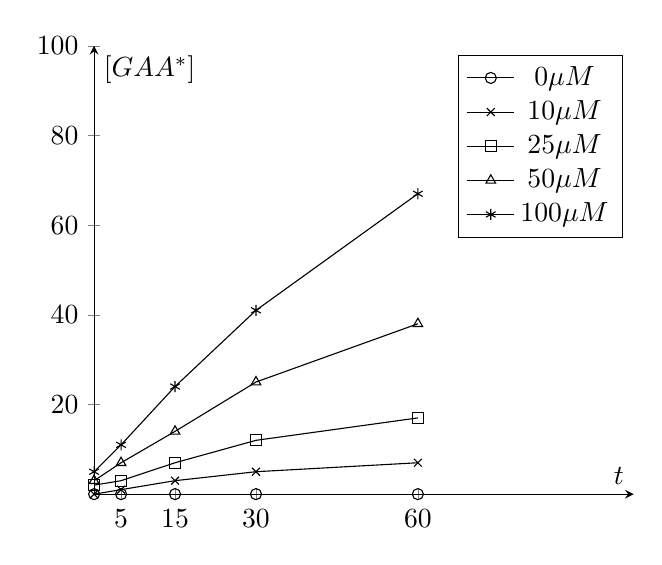
\begin{tikzpicture}
				\begin{axis}[axis lines=middle, xmin=0, xmax=100, ymin=0, ymax=100,samples=100, xtick={5, 15, 30, 60}, xlabel={$t$}, ylabel={$[GAA^*]$}]
				\addplot[
				scatter,
				point meta=explicit symbolic,
				scatter/classes={
					a={mark=o,draw=black},
					b={mark=x, draw=black},
					c={mark=square,draw=black},
					d={mark=triangle,draw=black},
					e={mark=asterisk,draw=black}}
				]
				table [meta=label]{
					x y label err
					0 0 a 1
					5 0 a 2
					15 0 a 3
					30 0 a 4
					60 0 a 5
				};
				\addplot[
				scatter,
				point meta=explicit symbolic,
				scatter/classes={
					a={mark=o,draw=black},
					b={mark=x, draw=black},
					c={mark=square,draw=black},
					d={mark=triangle,draw=black},
					e={mark=asterisk,draw=black}}
				]
				table [meta=label]{
					x y label
					0 0 b
					5 1 b
					15 3 b
					30 5 b
					60 7 b
				};
				\addplot[
				scatter,
				point meta=explicit symbolic,
				scatter/classes={
					a={mark=o,draw=black},
					b={mark=x, draw=black},
					c={mark=square,draw=black},
					d={mark=triangle,draw=black},
					e={mark=asterisk,draw=black}}
				]
				table [meta=label]{
					x y label
					0 2 c
					5 3 c
					15 7 c
					30 12 c
					60 17 c
				};
				\addplot[
				scatter,
				point meta=explicit symbolic,
				scatter/classes={
					a={mark=o,draw=black},
					b={mark=x, draw=black},
					c={mark=square,draw=black},
					d={mark=triangle,draw=black},
					e={mark=asterisk,draw=black}}
				]
				table [meta=label]{
					x y label
					0 3 d
					5 7 d
					15 14 d
					30 25 d
					60 38 d
				};
				\addplot[
				scatter,
				point meta=explicit symbolic,
				scatter/classes={
					a={mark=o,draw=black},
					b={mark=x, draw=black},
					c={mark=square,draw=black},
					d={mark=triangle,draw=black},
					e={mark=asterisk,draw=black}}
				]
				table [meta=label]{
					x y label
					0 5 e
					5 11 e
					15 24 e
					30 41 e
					60 67 e
				};
				
				
				
				\legend{$0\mu M$,$10\mu M$,$25\mu M$,$50\mu M$,$100\mu M$};
				
				\end{axis}
				\end{tikzpicture}
				\caption{Rate di ingresso del guanidinoacetato negli eritrociti a diverse concentrazioni}
				\label{fig:gaauptake}
			\end{figure}
	
	Per meglio caratterizzare la cinetica, \`e stato realizzato il diagramma dei doppi reciproci in figura \ref{fig:gaalineweaver}, ponendo in ascissa l'inverso delle concentrazioni e in ordinata l'inverso delle velocit\`a, calcolate come pendenza della retta di regressione lineare ottenuta sui punti di ognuna delle curve, ad eccezione della curva corrispondente a $0\mu M$ di guanidinoacetato esterno.
	\`E stata effettuata un'ulteriore regressione lineare sui punti per ottenere la retta di regressione:
	\begin{equation*}
		y = 48.9333 x + 0.0853333, \qquad(R^2 = 0.998832),
	\end{equation*}
	da cui \`e stata calcolata una costante $v\_uptake = 0.02 \mu M/min$.
		
		\begin{figure}
			\center
			\begin{tikzpicture}
			\begin{axis}[axis lines=middle, xmin=-0.01, xmax=0.1, ymin=-0.5, ymax=5,domain=-0.1:0.5,samples=100, xlabel={$\frac{1}{[S]}$}, ylabel={$\frac{1}{V}$}]
			\addplot[black]{48.9333*x + 0.0853333};
			\addplot[
			scatter,
			only marks,
			point meta=explicit symbolic,
			scatter/classes={
				a={mark=o,draw=black}}
			]
			table [meta=label]{
				x y label
				0.1 5 a
				0.04 2 a
				0.02 1 a
				0.01 0.66 a
			};
			
			\end{axis}
			\end{tikzpicture}
			\caption{Diagramma dei doppi reciproci dell'ingresso di guanidinoacetato negli eritrociti}
			\label{fig:gaalineweaver}
		\end{figure}
	
	\subsection{Esperimenti sul dosaggio della creatina prodotta}\label{sez:dosaggio}
		In un paziente GAMT deficiente, l'elevata disponibilit\`a di guanidinoacetato nel plasma si riflette in una cinetica potenzialmente elevata della GAMT incapsulata negli eritrociti.
		Oltre all'uptake di guanidinoacetato, l'altro elemento limitante pu\`o essere costituito dall'S-adenosil metionina, che rischia di non essere prodotta a velocit\`a sufficientemente elevata dalla SAMS eritrocitaria.
		
		Per verificare se sia necessario incapsulare, oltre alla GAMT, SAMS clonata da \emph{E.\ coli}, si sono effettuati esperimenti di dosaggio della creatina prodotta, a partire da quantit\`a preformate di S-adenosil metionina.
		
		Il sangue \`e stato centrifugato fino a ottenere tre aliquote di 780 $\mu l$ al \SI{90}{\percent} di ematocrito.
		Una delle aliquote \`e stata addizionata a 220 $\mu l$ di HEPES e funge da controllo, le altre due sono state addizionate ciascuna a 220 $\mu l$ di soluzione contenente 660 $\mu g$ di GAMT.
		Da ognuna sono stati prelevati \SI{50}{\micro l} e alle aliquote contenenti GAMT sono state aggiunte rispettivamente 2.5 $\mu l$ e 10 $\mu l$ di soluzione 5 $nM$ di S-adenosil metionina.
		Le due aliquote sono state processate tramite RCL per incapsulare GAMT e S-adenosil metionina, e, insieme all'aliquota controllo, sono state diluite fino a ottenere un ematocrito al \SI{50}{\percent}.
		
		Dalle tre soluzioni sono stati prelevati 250 $\mu l$ ed \`e stata verificata tramite HPLC la quantit\`a di S-adenosil metionina effettivamente incapsulata, ottenendo una concentrazione di circa 25 $\mu M$ per l'aliquota trattata con 2.5 $\mu l$ e 125 $\mu M$ per l'aliquota trattata con 10 $\mu l$.
		
		Sono stati aggiunti 7 $\mu l$ di soluzione contenente guanidinoacetato $^{13}C$ a concentrazione 5 $nM$ e si sono incubate le soluzioni a \SI{37}{\celsius}.
		Ai tempi 0, 1, 2, 3 e 20 ore sono stati prelevati 50 $\mu l$ di soluzione ed essiccati su cartoncino per bloccare le reazioni.
		
		L'analisi elettrospray ha prodotto le seguenti tabelle:
	\begin{table}[H]
		\centering
		\begin{tabular}{| c | c | c |}
			\hline
			Tempo (ore) & $[GAA]\ (\mu M)$ & $[Cr]\ (\mu M)$ \\
			\hline
			0 & 0.13 & 59.80\\
			\hline
			1 & 0.15 & 72.20\\
			\hline
			2 & 0.16 & 75.25\\
			\hline
			3 & 0.20 & 75.86\\
			\hline
			20 & 0.27 & 76.31\\
			\hline
		\end{tabular}
		\caption{Concentrazioni di guanidinoacetato e creatina in eritrociti non ingegnerizzati.}
		\label{tab:unloaded}
	\end{table}
	
	\begin{table}[H]
		\centering
		\begin{tabular}{| c | c | c |}
			\hline
			Tempo (ore) & $[GAA]\ (\mu M)$ & $[Cr]\ (\mu M)$ \\
			\hline
			0 & 2.61 & 66.01\\
			\hline
			1 & 3.10 & 61.90\\
			\hline
			2 & 4.62 & 63.37\\
			\hline
			3 & 5.11 & 67.50\\
			\hline
			20 & 5.26 & 59.31\\
			\hline
		\end{tabular}
		\caption{Concentrazioni di guanidinoacetato e creatina in eritrociti ingegnerizzati con GAMT e 25 $\mu M$ di SAM.}
		\label{tab:25um}
	\end{table}
	
	\begin{table}[H]
		\centering
		\begin{tabular}{| c | c | c |}
			\hline
			Tempo (ore) & $[GAA]\ (\mu M)$ & $[Cr]\ (\mu M)$ \\
			\hline
			0 & 7.32 & 66.32\\
			\hline
			1 & 10.52 & 64.55\\
			\hline
			2 & 13.87 & 65.87\\
			\hline
			3 & 12.18 & 61.58\\
			\hline
			20 & 15.13 & 59.88\\
			\hline
		\end{tabular}
		\caption{Concentrazioni di guanidinoacetato e creatina in eritrociti ingegnerizzati con GAMT e 125 $\mu M$ di SAM.}
		\label{tab:125um}
	\end{table}
